\documentclass[11pt]{report}

\usepackage[T1]{fontenc}
\usepackage[utf8]{inputenc}
\usepackage[sfdefault,lining]{FiraSans}
\renewcommand{\familydefault}{\sfdefault}
\usepackage{microtype}
\usepackage[margin=1in]{geometry}
\usepackage{amsmath,amssymb,mathtools}
\usepackage{booktabs}
\usepackage{array}
\usepackage{tabularx}
\usepackage{longtable}
\usepackage{multirow}
\usepackage{siunitx}
\usepackage{enumitem}
\usepackage{graphicx}
\usepackage{float}
\usepackage[table]{xcolor}
\usepackage{listings}
\usepackage{caption}
\usepackage{subcaption}
\usepackage{xurl}
\usepackage[hidelinks,pdfpagelabels=true,plainpages=false]{hyperref}
\usepackage{bookmark}
\usepackage[backend=biber,style=ieee,sorting=none,url=true,doi=true,isbn=false,eprint=true]{biblatex}
\usepackage{tikz}
\usetikzlibrary{arrows.meta,positioning,fit,shapes.geometric,shapes.misc}

\addbibresource{references.bib}

\captionsetup{font=small,labelfont=bf}
\setlength{\emergencystretch}{2em}
\setlength{\LTleft}{0pt}
\setlength{\LTright}{0pt}
\setlist[itemize]{leftmargin=1.5em}
\setlist[enumerate]{leftmargin=1.75em}
\setcounter{tocdepth}{2}
\renewcommand*{\bibfont}{\small}
\urlstyle{same}
\sisetup{detect-all=true}

\definecolor{cfblue}{HTML}{1F4E79}
\definecolor{cflight}{HTML}{EAF2F8}
\definecolor{cfcodebg}{HTML}{F7F9FB}
\definecolor{cfgray}{HTML}{58616A}

\newcolumntype{L}[1]{>{\raggedright\arraybackslash}p{#1}}
\newcolumntype{Y}{>{\raggedright\arraybackslash}X}

\lstdefinestyle{cfpython}{
  language=Python,
  basicstyle=\ttfamily\small,
  keywordstyle=\color{cfblue}\bfseries,
  commentstyle=\color{cfgray},
  stringstyle=\color{teal!60!black},
  showstringspaces=false,
  columns=fullflexible,
  keepspaces=true,
  frame=single,
  framerule=0.3pt,
  backgroundcolor=\color{cfcodebg},
  rulecolor=\color{black!20},
  breaklines=true,
  tabsize=2,
  captionpos=b
}

\lstdefinestyle{cfxml}{
  language=XML,
  basicstyle=\ttfamily\small,
  showstringspaces=false,
  columns=fullflexible,
  keepspaces=true,
  frame=single,
  framerule=0.3pt,
  backgroundcolor=\color{cfcodebg},
  rulecolor=\color{black!20},
  breaklines=true,
  captionpos=b
}

\DeclareRobustCommand{\codepath}[1]{\path{#1}}
\newcommand{\implnote}[1]{\par\smallskip\noindent\textbf{Implementation anchor.} #1\par\smallskip}
\newcommand{\heuristicnote}{\textbf{Heuristic note.} The scoring or mapping rule in this subsection is a repository implementation heuristic. It is documented here because it materially affects runtime behavior, not because it is claimed as a canonical external benchmark method.}

\title{A Research-Style Methodology of the \texttt{card-framework} Pipeline\\
\large Stage-1 Through Stage-4 Runtime\\
\large Affect Analysis and Tool Orchestration}
\author{Repository methodology document}
\date{Compiled on 2026-03-28}

\begin{document}

\pagenumbering{gobble}
\hypersetup{pageanchor=false}
\maketitle
\clearpage
\hypersetup{pageanchor=true}
\pagenumbering{roman}
\tableofcontents
\clearpage
\listoffigures
\clearpage
\listoftables
\clearpage
\pagenumbering{arabic}
\setcounter{page}{1}

\chapter{Scope and Defaults}

This document describes the implemented methodology of the \texttt{card-framework} repository as a staged pipeline from stage-1 through stage-4. The emphasis is the shipped code path, not a conceptual rewrite. The document therefore follows the actual runtime composition in \codepath{conf/config.yaml}, \codepath{src/card_framework/cli/main.py}, \codepath{src/card_framework/runtime/pipeline_plan.py}, and \codepath{src/card_framework/orchestration/stage_orchestrator.py}.

The most important default settings are summarized in Table~\ref{tab:default-runtime}. These defaults matter because they change what the methodology is in practice: the default run does not use embeddings, does run affect analysis, and does use live-draft audio so stage-2 duration control is based on actual rendered audio durations rather than a WPM proxy.

\begin{table}[H]
\centering
\small
\begin{tabularx}{\textwidth}{L{3.5cm}L{3.0cm}Y}
\toprule
Setting & Default value & Practical consequence \\
\midrule
\codepath{selection.llm} & \codepath{vllm_local} & The default runtime uses a local vLLM-compatible provider profile; benchmarking this profile requires separately identifying the backend model served behind it. \\
\codepath{selection.embedding} & \codepath{disabled} & Retrieval embeddings are disabled by default, so stage-2 uses full-transcript mode and does not expose \codepath{query_transcript} as an active tool. \\
\codepath{audio.affect_analysis.enabled} & \codepath{true} & Stage-1 and stage-2 transcripts are enriched with categorical and dimensional affect metadata, including direct emotion vectors. \\
\codepath{audio.voice_clone.enabled} & \codepath{true} & The accepted summary is rendered into cloned speaker audio unless the run is intentionally staged earlier. \\
\codepath{audio.voice_clone.live_drafting.enabled} & \codepath{true} & Mutating stage-2 tool calls render turn audio immediately; budget checks then use measured audio durations. \\
\codepath{orchestrator.duration_tolerance_ratio} & \codepath{0.05} & The runtime enforces a \(\pm 5\%\) duration tolerance band around the requested target duration. \\
\bottomrule
\end{tabularx}
\caption{Shipped default runtime settings most relevant to the methodology.}
\label{tab:default-runtime}
\end{table}

The overall dataflow is shown in Fig.~\ref{fig:pipeline-overview}.

\begin{figure}[H]
\centering
\resizebox{\textwidth}{!}{%
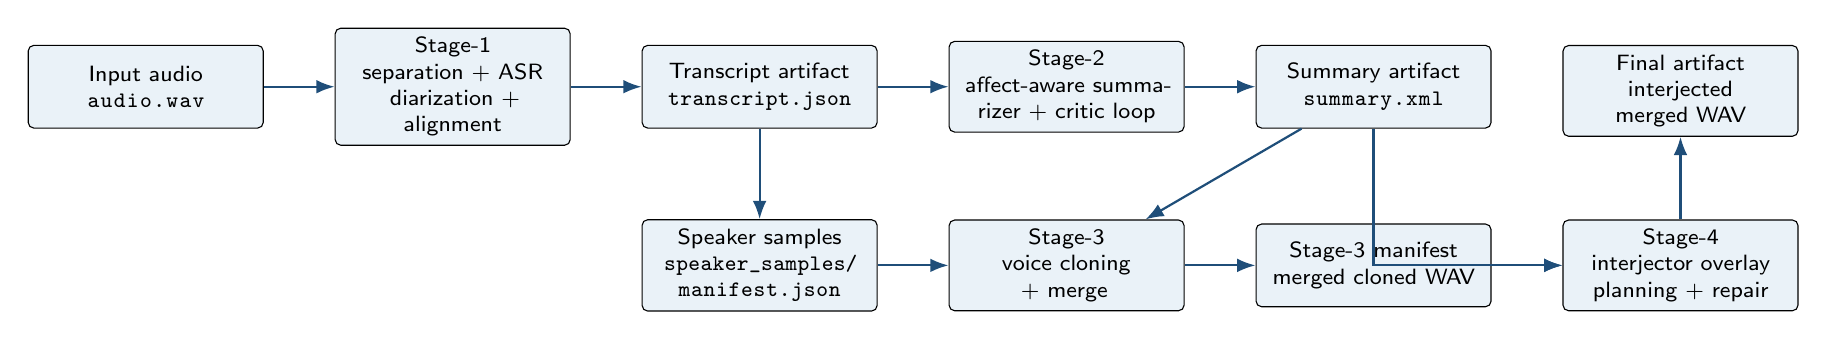
\begin{tikzpicture}[
  font=\footnotesize,
  node distance=0.95cm and 0.9cm,
  box/.style={draw, rounded corners=2pt, fill=cflight, align=center, text width=2.75cm, minimum height=1.05cm},
  arrow/.style={-Latex, thick, cfblue}
]
\node[box] (input) {Input audio\\\codepath{audio.wav}};
\node[box, right=of input] (stage1) {Stage-1\\separation + ASR\\diarization + alignment};
\node[box, right=of stage1] (transcript) {Transcript artifact\\\codepath{transcript.json}};
\node[box, right=of transcript] (stage2) {Stage-2\\affect-aware summarizer + critic loop};
\node[box, right=of stage2] (summary) {Summary artifact\\\codepath{summary.xml}};

\node[box, below=1.15cm of transcript] (samples) {Speaker samples\\\codepath{speaker_samples/}\\\codepath{manifest.json}};
\node[box, right=of samples] (stage3) {Stage-3\\voice cloning + merge};
\node[box, right=of stage3] (manifest) {Stage-3 manifest\\merged cloned WAV};
\node[box, right=of manifest] (stage4) {Stage-4\\interjector overlay planning + repair};
\node[box, above=1.05cm of stage4] (final) {Final artifact\\interjected merged WAV};

\draw[arrow] (input) -- (stage1);
\draw[arrow] (stage1) -- (transcript);
\draw[arrow] (transcript) -- (stage2);
\draw[arrow] (stage2) -- (summary);
\draw[arrow] (transcript) -- (samples);
\draw[arrow] (summary) -- (stage3);
\draw[arrow] (samples) -- (stage3);
\draw[arrow] (stage3) -- (manifest);
\draw[arrow] (summary) |- (stage4);
\draw[arrow] (manifest) -- (stage4);
\draw[arrow] (stage4) -- (final);
\end{tikzpicture}%
}
\caption{End-to-end pipeline implemented by the repository. Stage-2 can begin from an existing transcript, stage-3 from an existing summary, and stage-4 from an existing summary plus a stage-3 manifest.}
\label{fig:pipeline-overview}
\end{figure}

\chapter{Execution Modes and Artifact Contracts}

The stage entry policy is encoded in \codepath{src/card_framework/runtime/pipeline_plan.py}. The runtime accepts four start stages: \texttt{stage-1}, \texttt{stage-2}, \texttt{stage-3}, and \texttt{stage-4}. Table~\ref{tab:start-stages} summarizes the required inputs and outputs.

\begin{table}[H]
\centering
\small
\begin{tabularx}{\textwidth}{L{1.5cm}L{3.2cm}L{4.4cm}Y}
\toprule
Start stage & Required existing artifact(s) & Executed components & Principal output(s) \\
\midrule
\texttt{stage-1} & input audio & stage-1, stage-2, optional stage-3, optional stage-4 & transcript, summary, optional cloned audio, optional interjected audio \\
\texttt{stage-2} & transcript JSON & stage-2, optional stage-3, optional stage-4 & summary, optional cloned audio, optional interjected audio \\
\texttt{stage-3} & summary XML and transcript metadata that resolves speaker samples & stage-3, optional stage-4 & stage-3 manifest and merged cloned audio, optional stage-4 output \\
\texttt{stage-4} & summary XML plus stage-3 manifest & stage-4 only & interjector manifest and final interjected merged audio \\
\bottomrule
\end{tabularx}
\caption{Execution modes accepted by the runtime.}
\label{tab:start-stages}
\end{table}

The principal serialized contracts are:

\begin{itemize}
  \item \textbf{Transcript JSON:} top-level \codepath{segments} plus \codepath{metadata}, represented at runtime by \codepath{src/card_framework/orchestration/transcript.py}. Extra segment keys are preserved, which is essential for affect metadata and overlap metadata.
  \item \textbf{Summary XML:} speaker-tagged XML turns represented by \codepath{src/card_framework/shared/summary_xml.py}. New outputs are vector-first and can carry \codepath{emotion_vector}, \codepath{emotion_vector_source}, \codepath{source_segment_indices}, and \codepath{source_segment_weights}.
  \item \textbf{Speaker-sample manifest:} generated by \codepath{src/card_framework/audio_pipeline/speaker_samples.py}; it records selected slices, target duration, audio format, and output paths.
  \item \textbf{Voice-clone manifest:} generated by stage-3; it records one synthesized artifact per summary turn and the optional merged WAV.
  \item \textbf{Interjector manifest:} generated by stage-4; it records accepted and rejected overlays, timing source, timing variant, repair history, and overlay-fit telemetry.
\end{itemize}

Listing~\ref{lst:summaryxml} shows the downstream summary shape used by stage-3 and stage-4.

\begin{lstlisting}[style=cfxml,caption={Representative summary XML shape used downstream by stage-3 and stage-4. Adapted from \codepath{src/card_framework/shared/summary_xml.py}.},label={lst:summaryxml}]
<SPEAKER_00 emotion_categories="calm,warm"
            emotion_vector="0.060,0.000,0.020,0.000,0.000,0.090,0.010,0.310"
            emotion_vector_source="source_linked"
            source_segment_indices="17,18,19"
            source_segment_weights="0.410000,0.360000,0.230000">
  The host reframes the episode around recovery, isolation, and renewed purpose.
</SPEAKER_00>
<SPEAKER_01 emotion_categories="surprised,upbeat,calm"
            emotion_vector="0.140,0.000,0.000,0.000,0.000,0.030,0.220,0.180"
            emotion_vector_source="explicit">
  The guest answers with a more vivid, more personal version of the same arc.
</SPEAKER_01>
\end{lstlisting}

\implnote{Transcript DTOs are defined in \codepath{src/card_framework/orchestration/transcript.py}; A2A request/response DTOs are defined in \codepath{src/card_framework/agents/dtos.py}; summary XML parsing and serialization are implemented in \codepath{src/card_framework/shared/summary_xml.py}.}

\chapter{Stage-1: Audio Front-End and Affect Analysis}

\section{Operational decomposition}

Stage-1 is implemented by \codepath{src/card_framework/audio_pipeline/orchestrator.py}. Its core sequence is deterministic: source separation, speech recognition, diarization, alignment, optional affect analysis, then atomic transcript emission.

\begin{table}[H]
\centering
\small
\begin{tabularx}{\textwidth}{L{3.2cm}L{3.3cm}Y}
\toprule
Subsystem & Default setting(s) & Role in the pipeline \\
\midrule
Source separation & \codepath{provider=demucs}, \codepath{model=htdemucs}, window \(600\) s, context \(5\) s & Removes accompaniment and bounds memory use by separating long audio in windows. \\
ASR & \codepath{granite_speech}, chunk length \(25\) s, overlap \(1\) s, \codepath{max_new_tokens=96}, repetition penalty \(1.25\) & Produces segment text and, when available, word timestamps for word-level speaker alignment. \\
Diarization & \codepath{diar_msdd_telephonic}, \codepath{titanet_large}, \codepath{vad_multilingual_marblenet}, \codepath{max_speakers=10} & Produces speaker turns with overlap-aware behavior retained for downstream metadata. \\
Affect analysis & categorical: \codepath{emotion2vec_plus_large}; dimensional: \codepath{audeering/wav2vec2-large-robust-12-ft-emotion-msp-dim} & Enriches transcript segments with affect hints, preset suggestions, and direct 8D emotion vectors. \\
\bottomrule
\end{tabularx}
\caption{Default stage-1 front-end configuration.}
\label{tab:stage1-defaults}
\end{table}

\section{Stage-1 timing model}

Stage-1 ETA starts from configured per-stage throughput multipliers and is then refined online. If an audio file has duration \(D\) seconds and the configured stage multiplier is \(m_{s,d}\) for stage \(s\) and device \(d\), the initial estimate is

\begin{equation}
\hat{T}_{s,0} = D \cdot m_{s,d}.
\end{equation}

Observed throughput then updates the stored multiplier with exponential smoothing,

\begin{equation}
m_{k+1} = (1 - \alpha)m_k + \alpha m_{\mathrm{obs}},
\end{equation}

where \(\alpha\) is the configured learning rate in \codepath{conf/config.yaml}. This is a runtime control heuristic, not a benchmark metric.

\section{ASR, diarization, and alignment}

If Granite returns word timestamps, stage-1 performs word-level speaker alignment first; otherwise it falls back to segment-level alignment.

\begin{lstlisting}[style=cfpython,caption={Condensed stage-1 orchestration flow adapted from \codepath{src/card_framework/audio_pipeline/orchestrator.py}.},label={lst:stage1flow}]
vocals_path = separator.separate_vocals(...)
asr_result = transcriber.transcribe(vocals_path, ...)
diarization_turns = diarizer.diarize(vocals_path, ...)

if asr_result.word_timestamps:
    aligned_segments = build_word_speaker_segments(
        word_timestamps=asr_result.word_timestamps,
        diarization_turns=diarization_turns,
        default_speaker=default_speaker,
        merge_gap_ms=merge_gap_ms,
    )
else:
    aligned_segments = align_segments_with_speakers(
        asr_segments=asr_result.segments,
        diarization_turns=diarization_turns,
        default_speaker=default_speaker,
        merge_gap_ms=merge_gap_ms,
    )

write_transcript_atomic(payload, output_transcript_path)
\end{lstlisting}

\section{Default affect-analysis algorithm}

Affect analysis is enabled by default and runs after transcript availability. The implementation is centered on \codepath{src/card_framework/audio_pipeline/affect_analysis.py}. It prepares one audio clip per transcript segment, runs a categorical provider (emotion2vec+) and a dimensional provider (audEERING MSP-dim), merges their outputs, derives both a prompt-facing preset hint and a direct 8D IndexTTS emotion vector, and writes the resulting metadata back onto the transcript under keys such as \codepath{affect}, \codepath{affect_hint}, \codepath{suggested_emo_preset}, \codepath{emotion_vector}, \codepath{emotion_vector_source}, and \codepath{emotion_vector_confidence}.

For a segment with categorical labels \((\ell_k, s_k)\), arousal \(a\), dominance \(d\), and valence \(v\), the mapper first accumulates categorical evidence into the IndexTTS basis with categorical weight \(w_c = 0.65\):

\begin{equation}
u_j = \sum_{k : m(\ell_k)=j} w_c s_k,
\end{equation}

where \(m(\cdot)\) is the repository alias map from provider labels onto the IndexTTS emotion basis.

The dimensional provider then contributes with weight \(w_d = 0.35\). Let \(d' = d\) when dominance is present and \(d'=0.5\) otherwise. The implemented updates are

\begin{align}
q_{\text{happy}} &= v (0.45 + 0.55 a) w_d, \\
q_{\text{surprised}} &= v a \beta_{\text{surprise}} w_d, \\
q_{\text{calm}} &= (1-a)(0.3 + 0.7 v) w_d, \\
q_{\text{melancholic}} &= (1-v)(1-a) \beta_{\text{mel}} w_d, \\
q_{\text{sad}} &= (1-v)(1-a)(0.45 + 0.35(1-d')) w_d, \\
q_{\text{angry}} &= (1-v) a d' \beta_{\text{ang}} w_d, \\
q_{\text{afraid}} &= (1-v) a (1-d') \beta_{\text{fear}} w_d, \\
q_{\text{disgusted}} &= (1-v)(0.25 + 0.75 d') \beta_{\text{disg}} w_d.
\end{align}

With shipped defaults,
\(\beta_{\text{surprise}}=0.35\),
\(\beta_{\text{ang}}=0.85\),
\(\beta_{\text{fear}}=0.9\),
\(\beta_{\text{mel}}=0.7\), and
\(\beta_{\text{disg}}=0.35\).

After adding a calm floor \(\gamma = 0.12\), the vector is capped and normalized in two stages. First, if any component exceeds the dominant-emotion cap \(\kappa = 0.38\), the full vector is rescaled by \(\kappa / \max_j x_j\). Second, the IndexTTS bias vector \(\mathbf{b}\) from \codepath{src/card_framework/shared/emotion_vector.py} is applied and the total intensity is clamped to \(M = 0.8\):

\begin{equation}
x_j = \max(0, u_j + q_j + \delta_j), \qquad
\tilde{x}_j = b_j x_j, \qquad
e_j = \tilde{x}_j \cdot \min\left(1, \frac{M}{\sum_i \tilde{x}_i}\right),
\end{equation}

where \(\delta_{\text{calm}}=\gamma\) and \(\delta_j=0\) otherwise.

The confidence score stored with the vector is likewise heuristic and conservative:

\begin{equation}
c = \max\left(c_{\min}, \min\left(1, \max\left(\max_k s_k, 0.5 + 0.5|0.5-v|\right)\right)\right),
\end{equation}

with confidence floor \(c_{\min}=0.15\).

The preset hint is computed separately through threshold rules. With allowed presets \(\{\text{urgent}, \text{upbeat}, \text{warm}, \text{engaged}, \text{neutral}\}\), the shipped decision rules are

\begin{equation}
\text{preset} =
\begin{cases}
\text{urgent}, & \ell_1 \in \mathcal{U} \; \text{or} \; a \ge 0.65, \\
\text{upbeat}, & \ell_1 \in \mathcal{B} \; \text{or} \; v \ge 0.60, \\
\text{warm}, & v \ge 0.48 \; \wedge \; a \le 0.45, \\
\text{engaged}, & a \ge 0.45, \\
\text{neutral}, & \text{otherwise.}
\end{cases}
\end{equation}

Here \(\mathcal{U}=\{\text{angry},\text{fearful}\}\) and \(\mathcal{B}=\{\text{happy},\text{surprised}\}\). The preset is therefore a prompt-facing abstraction, whereas the voice-clone path itself uses the explicit vector when present.

\begin{table}[H]
\centering
\small
\begin{tabular}{lcc}
\toprule
Coefficient & Symbol & Default value \\
\midrule
categorical weight & \(w_c\) & 0.65 \\
dimensional weight & \(w_d\) & 0.35 \\
calm floor & \(\gamma\) & 0.12 \\
surprise boost & \(\beta_{\text{surprise}}\) & 0.35 \\
anger bias & \(\beta_{\text{ang}}\) & 0.85 \\
fear bias & \(\beta_{\text{fear}}\) & 0.90 \\
melancholic bias & \(\beta_{\text{mel}}\) & 0.70 \\
disgust bias & \(\beta_{\text{disg}}\) & 0.35 \\
confidence floor & \(c_{\min}\) & 0.15 \\
dominant-emotion cap & \(\kappa\) & 0.38 \\
vector max sum & \(M\) & 0.80 \\
\bottomrule
\end{tabular}
\caption{Default affect-to-vector mapping coefficients from \codepath{conf/config.yaml}.}
\label{tab:affect-coeffs}
\end{table}

\begin{lstlisting}[style=cfpython,caption={Condensed affect-analysis merge path adapted from \codepath{src/card_framework/audio_pipeline/affect_analysis.py}.},label={lst:affectmerge}]
suggested_emo_preset = _suggest_emo_preset(...)
emotion_vector_result = self.emotion_vector_mapping.map(
    emotion_scores=top_scores,
    arousal=arousal,
    dominance=dominance,
    valence=valence,
)
extras["affect"] = record.to_payload()
extras["affect_hint"] = record.hint
extras["suggested_emo_preset"] = record.suggested_emo_preset
extras["emotion_vector"] = record.emotion_vector.to_list()
extras["emotion_vector_source"] = record.emotion_vector_source
extras["emotion_vector_confidence"] = record.emotion_vector_confidence
\end{lstlisting}

\heuristicnote

\section{Public benchmark positioning of default stage-1 models}

\subsection{Exact or directly accessible checkpoint evidence}

\begin{table}[H]
\centering
\scriptsize
\begin{tabularx}{\textwidth}{L{2.0cm}L{2.5cm}L{1.2cm}L{1.5cm}L{2.1cm}L{1.3cm}}
\toprule
Component & Benchmark & Metric & Score & Base & Base score \\
\midrule
Granite Speech & vendor aggregate & Average WER / RTFx & 5.52 / 280.02 & Parakeet TDT 0.6B v2 & 6.05 / 3380 \\
MSDD telephonic & CH109 fair & DER & 3.52\% & n/a & n/a \\
TitaNet Large & VoxCeleb1 & EER & 0.66\% & n/a & n/a \\
MarbleNet multilingual VAD & AVA Speech ALL & AUROC / TPR & 0.9112 / 0.9093 & n/a & n/a \\
\bottomrule
\end{tabularx}
\caption{Public benchmark positioning for the main default stage-1 speech front-end components. Where no matched external baseline on the same accessible benchmark was located for the exact default component, the baseline fields are left blank rather than filled with a cross-dataset proxy.}
\label{tab:stage1-public}
\end{table}

For the VAD row in Table~\ref{tab:stage1-public}, the reported true-positive rate is measured at a fixed false-positive rate of 0.315 on AVA Speech [\cite{marblenet_vad_modelcard}].

\subsection{Family-level or partial public evidence}

\begin{table}[H]
\centering
\scriptsize
\begin{tabularx}{\textwidth}{L{2.8cm}L{1.8cm}L{1.4cm}L{1.2cm}L{2.6cm}L{1.2cm}}
\toprule
Affect model & Benchmark & Metric & Score & Base & Base score \\
\midrule
emotion2vec+ family & MELD & WA & 51.88 & data2vec 2.0 & 48.92 \\
emotion2vec+ family & RAVDESS & WA & 82.43 & data2vec 2.0 & 81.04 \\
audEERING MSP-dim family & MSP-Podcast & Valence CCC & 0.638 & Wav2Small teacher & 0.676 \\
\bottomrule
\end{tabularx}
\caption{Public benchmark positioning for the default affect-analysis models. The emotion2vec row is family-level because the exact plus-large checkpoint table was not publicly enumerated; the audEERING row is tied to the released MSP-dimensional checkpoint family.}
\label{tab:affect-public}
\end{table}

\begin{table}[H]
\centering
\scriptsize
\begin{tabularx}{\textwidth}{L{2.3cm}L{2.4cm}L{1.4cm}L{1.5cm}Y}
\toprule
Model family & Benchmark & Metric & Reported score & Why it remains family-level or partial evidence \\
\midrule
Demucs \codepath{htdemucs} family & MUSDB-HQ test & SDR & 9.0 dB; baseline Hybrid Demucs v3 7.7 dB & The accessible public comparison is reported at the Hybrid Transformer Demucs family level rather than as a separately benchmarked literal \codepath{htdemucs} artifact row. \\
emotion2vec+ family & MELD / RAVDESS & WA & 51.88 / 82.43 & The public exact numeric table is for the \codepath{emotion2vec} family paper, not the exact \codepath{emotion2vec_plus_large} checkpoint. \\
audEERING MSP-dim family & MSP-Podcast & Valence CCC & 0.638 & Public evidence is tied to the released MSP-dimensional system family; the exact checkpoint card does not expose a full matched benchmark table in the retrieved sources. \\
\bottomrule
\end{tabularx}
\caption{Family-level or partial public evidence used by default stage-1 and affect-analysis components.}
\label{tab:stage1-family-evidence}
\end{table}

\section{Repository-local tuning evidence}

\begin{table}[H]
\centering
\small
\begin{tabularx}{\textwidth}{L{2.4cm}L{2.7cm}L{2.2cm}L{2.2cm}Y}
\toprule
Area & Metric & Baseline & Promoted / improved & Internal source \\
\midrule
Granite tuning & adjacent-repeat segments & 34 & 14 & \cite{internal_granite_tuning_20260318} \\
Granite tuning & boundary seam candidates & 32 & 7 & \cite{internal_granite_tuning_20260318} \\
NeMo tuning & transcript sandwich candidates & 103 & 33 & \cite{internal_nemo_tuning_20260318} \\
NeMo tuning & short RTTM turns (\(\le 0.5\) s) & 69 in exact-7 oracle trial & 45 in promoted rerun & \cite{internal_nemo_tuning_20260318} \\
\bottomrule
\end{tabularx}
\caption{Repository-local empirical tuning evidence for stage-1 defaults.}
\label{tab:stage1-internal}
\end{table}

\chapter{Stage-2: Summarizer--Critic Orchestration}

\section{A2A architecture}

Stage-2 is the control center of the repository. A \texttt{StageOrchestrator} launches the summarizer--critic loop, optionally indexes transcript embeddings, prepares live-draft state and speaker samples, then persists the accepted \codepath{summary.xml}. Under the shipped defaults, embeddings are disabled, so retrieval indexing is bypassed and the full transcript is given directly to the summarizer and critic.

\begin{figure}[H]
\centering
\resizebox{0.96\textwidth}{!}{%
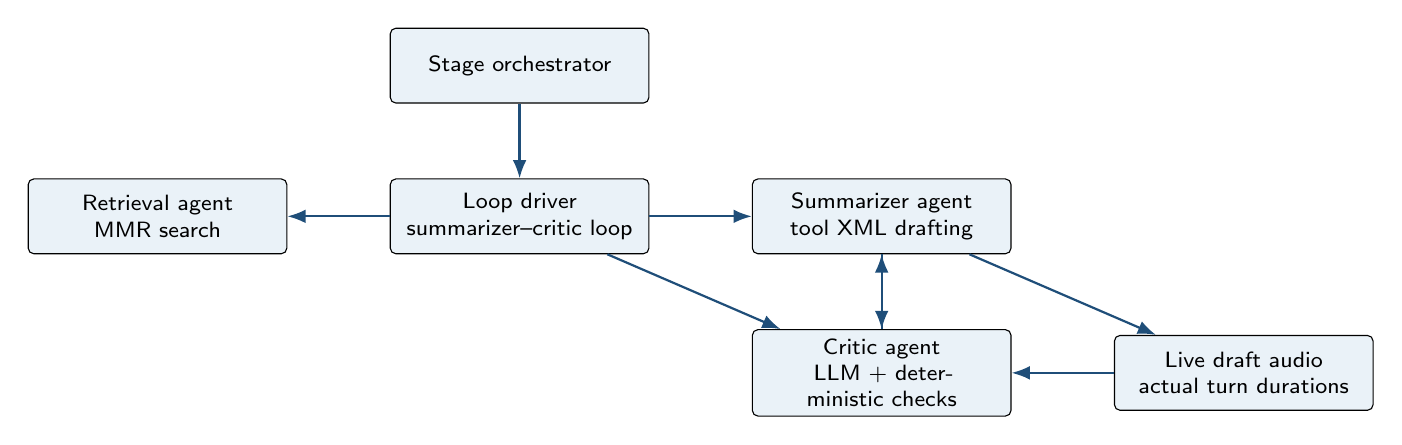
\begin{tikzpicture}[
  font=\footnotesize,
  node distance=0.95cm and 1.3cm,
  box/.style={draw, rounded corners=2pt, fill=cflight, align=center, text width=3.05cm, minimum height=0.95cm},
  arrow/.style={-Latex, thick, cfblue}
]
\node[box] (stage) {Stage orchestrator};
\node[box, below=of stage] (loop) {Loop driver\\summarizer--critic loop};
\node[box, left=of loop] (retrieval) {Retrieval agent\\MMR search};
\node[box, right=of loop] (summ) {Summarizer agent\\tool XML drafting};
\node[box, below=of summ] (critic) {Critic agent\\LLM + deterministic checks};
\node[box, right=of critic] (live) {Live draft audio\\actual turn durations};

\draw[arrow] (stage) -- (loop);
\draw[arrow] (loop) -- (retrieval);
\draw[arrow] (loop) -- (summ);
\draw[arrow] (loop) -- (critic);
\draw[arrow] (summ) -- (critic);
\draw[arrow] (critic) -- (summ);
\draw[arrow] (summ) -- (live);
\draw[arrow] (live) -- (critic);
\end{tikzpicture}%
}
\caption{Stage-2 local A2A topology. Retrieval is only active when embeddings are enabled. Under the shipped defaults, the summarizer and critic operate in full-transcript mode and use actual live-draft audio durations.}
\label{fig:a2a-loop}
\end{figure}

\section{Summarizer tool registry and policies}

The stage-2 summarizer does not generate the final XML in one unconstrained pass. It operates through an explicit tool registry assembled in \codepath{src/card_framework/agents/tool_handlers.py} and dispatched in \codepath{src/card_framework/agents/summarizer_tool_dispatcher.py}. The active tools are listed in Table~\ref{tab:summarizer-tools}.

\begin{table}[H]
\centering
\footnotesize
\begin{tabularx}{\textwidth}{L{3.2cm}Y L{2.4cm}}
\toprule
Tool & Purpose & Default availability \\
\midrule
\codepath{add_speaker_message} & Append one speaker turn, optionally with an explicit 8D emotion vector; in live-draft mode this immediately synthesizes turn audio. & yes \\
\codepath{edit_message} & Replace the content of one existing line and optionally replace its emotion vector; re-renders that turn in live-draft mode when needed. & yes \\
\codepath{remove_message} & Remove one line and delete its live-draft artifact when present. & yes \\
\codepath{estimate_duration} & Return current duration telemetry. With live drafting enabled this uses actual rendered audio, not WPM estimation. & yes \\
\codepath{count_words} & Return total word count, per-line counts, and per-speaker totals. & yes \\
\codepath{query_transcript} & Retrieve transcript segments via the retrieval agent. & only when embeddings are enabled \\
\codepath{save_draft} & Snapshot the current registry state into XML. & yes \\
\codepath{finalize_draft} & Declare the current draft ready for critic evaluation. & yes \\
\bottomrule
\end{tabularx}
\caption{Summarizer tools exposed to the LLM.}
\label{tab:summarizer-tools}
\end{table}

The dispatcher then enforces orchestration rules that materially shape model behavior:

\begin{itemize}
  \item only one mutating tool call is executed per assistant turn;
  \item replay-deduplication and mutation fingerprints are used to detect repeated no-op or oscillatory edits;
  \item once the draft is within budget, the runtime auto-saves the draft and injects a review-only turn that requires either \codepath{finalize_draft()} or one more mutating action;
  \item staged discovery can require multiple successful \codepath{query_transcript} calls before mutation or finalization, but this guardrail is only relevant when embeddings are enabled and the provider/model matches the configured guardrail predicates.
\end{itemize}

\section{Duration-first control with actual audio by default}

The accepted-duration band is defined by a target duration \(t\) and tolerance ratio \(r\):

\begin{equation}
\tau = tr, \qquad [t_{\min}, t_{\max}] = [t - \tau, t + \tau].
\label{eq:durationband}
\end{equation}

Under the shipped defaults, live drafting is enabled, so the draft duration used by \codepath{estimate_duration} and later critic checks is the sum of actual synthesized turn durations,

\begin{equation}
T_{\mathrm{draft}} = \sum_{i=1}^{n} \frac{d_i}{1000},
\end{equation}

where \(d_i\) is the measured duration in milliseconds of rendered turn \(i\). The runtime still records a per-turn actual WPM statistic for diagnostics,

\begin{equation}
\mathrm{actual\_wpm} = \frac{w}{d_{\mathrm{ms}} / 1000} \cdot 60,
\end{equation}

but that is not the primary budget estimator under the default path.

The summarizer timeout floor is also raised in live-draft mode:

\begin{equation}
T_{\mathrm{summ}} = \max(1800, 6t),
\end{equation}

where \(t\) is the requested target duration in seconds.

\begin{lstlisting}[style=cfpython,caption={Condensed stage-2 loop adapted from \codepath{src/card_framework/runtime/loop_orchestrator.py}.},label={lst:stage2loop}]
while max_iterations is None or iteration < max_iterations:
    summarizer_task = SummarizerTaskRequest(...)
    draft = await agent_client.send_task(summarizer_port, summarizer_task)

    critic_task = CriticTaskRequest(...)
    verdict = CriticTaskResponse.model_validate_json(
        await agent_client.send_task(critic_port, critic_task)
    )

    if verdict.status == "pass":
        return draft
    feedback = verdict.feedback
\end{lstlisting}

\section{Retrieval mode and MMR}

When a real embedding provider is configured, transcript segments are indexed and retrieved with maximal marginal relevance (MMR),

\begin{equation}
\mathrm{MMR}(d) = \lambda \, \mathrm{sim}(q,d) - (1-\lambda)\max_{s \in S}\mathrm{sim}(d,s),
\end{equation}

where \(q\) is the query, \(d\) is a candidate document segment, and \(S\) is the already selected set [\cite{carbonell1998mmr}]. The implementation lives in \codepath{src/card_framework/retrieval/embeddings.py}. Under the shipped defaults, however, embeddings are disabled and both summarizer and critic receive the full transcript text directly.

\section{Default benchmark comparison: embeddings enabled vs disabled}

Because embeddings are disabled by default, the most relevant internal stage-2 comparison is the matched enabled-vs-disabled SPoRC duration sweep pair run with 100 examples per preset, transcript-only mode, seed 42, and the same \codepath{vllm_default} summarizer, critic, and judge [\cite{internal_sporc_duration_sweep_enabled_20260319,internal_sporc_duration_sweep_20260320}]. Table~\ref{tab:embedding-compare} shows the result.

\begin{table}[H]
\centering
\footnotesize
\begin{tabular}{lcccccc}
\toprule
Preset & En. comp. & Dis. comp. & Delta & En. restarts & Dis. restarts & Tol. ok \\
\midrule
30s & 0.502 & 0.551 & +0.049 & 1 & 7 & 1.000 / 1.000 \\
1m & 0.505 & 0.627 & +0.122 & 0 & 10 & 1.000 / 1.000 \\
5m & 0.471 & 0.630 & +0.159 & 1 & 14 & 1.000 / 1.000 \\
\bottomrule
\end{tabular}
\caption{Matched 100-example SPoRC comparison between embeddings enabled and disabled. The shipped default is the disabled condition.}
\label{tab:embedding-compare}
\end{table}

The default-disabled result is also replicated by a second 100-example disabled sweep with composite scores 0.583, 0.620, and 0.638 for 30 seconds, 1 minute, and 5 minutes respectively [\cite{internal_sporc_duration_sweep_disabled_20260320b}].

The repository also contains a judge-only sweep over QMSum reference summaries [\cite{internal_faithful_judge_sweep_20260313}]. Table~\ref{tab:judge-sweep} captures its main quantitative result.

\begin{table}[H]
\centering
\small
\begin{tabular}{lcccc}
\toprule
Judge model & Candidate win rate & Mean overall & Errors & Wall clock (s) \\
\midrule
Qwen3.5-27B & 0.9800 & 0.6021 & 0 & 417.9 \\
Qwen3.5-9B & 0.7778 & 0.5722 & 1 & 401.8 \\
Qwen3.5-4B & 0.8427 & 0.5515 & 11 & 278.6 \\
\bottomrule
\end{tabular}
\caption{Repository-local faithful-judge sweep over 100 QMSum cases per model.}
\label{tab:judge-sweep}
\end{table}

\chapter{Stage-3: Voice Cloning and Summary Realization}

\section{Speaker-sample preparation and realization path}

Stage-3 consumes \codepath{summary.xml} and the speaker-sample manifest. In live-draft mode it can finalize already rendered turn-level audio without re-synthesizing every turn. Otherwise it performs a batch stage-3 render from the accepted summary. The batch path is implemented in \codepath{src/card_framework/audio_pipeline/voice_clone_orchestrator.py}; the incremental path is implemented in \codepath{src/card_framework/audio_pipeline/live_draft_voice_clone.py}.

\begin{table}[H]
\centering
\small
\begin{tabular}{lcc}
\toprule
Speaker-sample parameter & Default value & Meaning \\
\midrule
target duration per speaker & 30 s & Target sample length for each speaker reference \\
max slices & 6 & Maximum selected clean slices per speaker \\
minimum slice duration & 1200 ms & Lower bound for eligible source slices \\
sample rate & 44100 Hz & Export rate for generated speaker references \\
codec & \codepath{pcm_s24le} & Output format for speaker sample WAVs \\
\bottomrule
\end{tabular}
\caption{Default speaker-sample generation settings.}
\label{tab:speaker-samples}
\end{table}

When post-render verification is enabled, the stage-3 export is checked again against the stage-2 target using the same tolerance band from Eq.~\ref{eq:durationband}. If a merged stage-3 output exists, it is probed directly; otherwise durations are summed over per-turn artifacts.

\section{Public benchmark positioning of the TTS family}

The repository uses the IndexTTS family for voice cloning. Table~\ref{tab:tts-public} summarizes the public comparison extracted from the IndexTTS paper [\cite{indextts2025,indextts_repo}].

\begin{table}[H]
\centering
\small
\begin{tabular}{lccc}
\toprule
System & Avg WER/CER & Avg speaker similarity & Avg MOS \\
\midrule
IndexTTS & 3.7 & 0.776 & 4.01 \\
XTTS & 6.0 & 0.663 & 3.11 \\
CosyVoice2 & 5.9 & 0.788 & 3.81 \\
F5-TTS & 8.2 & 0.779 & 3.66 \\
FishSpeech & 8.3 & 0.612 & 3.57 \\
\bottomrule
\end{tabular}
\caption{Public zero-shot TTS comparison reported by the IndexTTS paper.}
\label{tab:tts-public}
\end{table}

\section{Repository-local end-to-end duration evidence}

An internal SPoRC DeepSeek bundle covering 15 outputs across five episodes and three duration presets records concrete final durations for all stage-3/stage-4 outputs [\cite{internal_deepseek_bundle_20260324}]. Table~\ref{tab:stage3-duration-bundle} summarizes the observed range by preset.

\begin{table}[H]
\centering
\small
\begin{tabular}{lccc}
\toprule
Target preset & Count & Min observed duration (s) & Max observed duration (s) \\
\midrule
30s & 5 & 29.246 & 31.498 \\
1m & 5 & 58.375 & 62.322 \\
5m & 5 & 268.158 & 293.236 \\
\bottomrule
\end{tabular}
\caption{Observed final durations in the repository-local 15-output SPoRC DeepSeek bundle.}
\label{tab:stage3-duration-bundle}
\end{table}

\chapter{Stage-4: Interjector Planning, Alignment, and Repair}

\section{Purpose and repair flow}

Stage-4 adds short overlapping backchannels or echo agreements from the next speaker onto the merged stage-3 audio. It is implemented in \codepath{src/card_framework/audio_pipeline/interjector.py}. The system uses summary-aware anchor spans, host-turn alignment, optional Faster-Whisper-native phrase matching for echo agreements, loudness-normalized overlay synthesis, and a repair loop that shortens or tightens candidates when they would violate the legal overlap window.

\begin{figure}[H]
\centering
\resizebox{0.95\textwidth}{!}{%
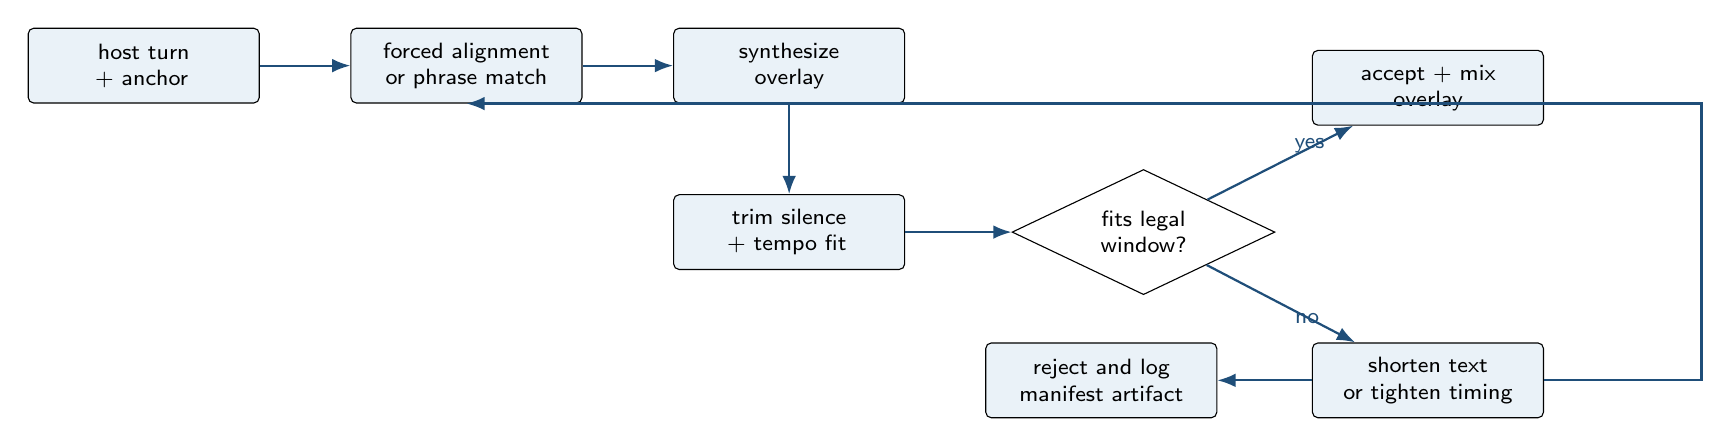
\begin{tikzpicture}[
  font=\footnotesize,
  node distance=1.1cm and 1.15cm,
  box/.style={draw, rounded corners=2pt, fill=cflight, align=center, text width=2.7cm, minimum height=0.95cm},
  arrow/.style={-Latex, thick, cfblue},
  decision/.style={diamond, draw, fill=white, aspect=2.1, align=center, inner sep=1.5pt, text width=1.9cm}
]
\node[box] (host) {host turn\\+ anchor};
\node[box, right=of host] (align) {forced alignment\\or phrase match};
\node[box, right=of align] (synth) {synthesize\\overlay};
\node[box, below=1.15cm of synth] (prep) {trim silence\\+ tempo fit};
\node[decision, right=1.35cm of prep] (fit) {fits legal\\window?};
\node[box, above right=0.95cm and 1.3cm of fit] (accept) {accept + mix\\overlay};
\node[box, below right=1.0cm and 1.3cm of fit] (repair) {shorten text\\or tighten timing};
\node[box, left=1.2cm of repair] (reject) {reject and log\\manifest artifact};

\draw[arrow] (host) -- (align);
\draw[arrow] (align) -- (synth);
\draw[arrow] (synth) -- (prep);
\draw[arrow] (prep) -- (fit);
\draw[arrow] (fit) -- node[above right, xshift=0.05cm] {yes} (accept);
\draw[arrow] (fit) -- node[below right, xshift=0.05cm] {no} (repair);
\draw[arrow] (repair.east) -- ++(2.0,0) |- (align.south);
\draw[arrow] (repair) -- (reject);
\end{tikzpicture}%
}
\caption{Stage-4 overlay repair loop. The implementation iterates over repair states until either the overlay fits the legal window or the reachable states are exhausted.}
\label{fig:stage4repair}
\end{figure}

\section{Timing equations}

The simplest hard constraint is the overlap fit test,

\begin{equation}
\text{fits} \iff d_{\mathrm{overlay}} \leq d_{\mathrm{available}}.
\end{equation}

For short echo agreements, the implementation also tries to align the overlay phrase with a matched host phrase. The phrase matcher uses an internal similarity score

\begin{equation}
\mathrm{score} = 0.7\,\mathrm{SeqSim}(\text{target}, \text{window}) + 0.3\,\mathrm{BoundarySim}(\text{target}, \text{window}),
\end{equation}

then tempo-fits the overlay if the phrase overflows the host phrase duration budget. If the host phrase duration is \(d_h\), the target host fill ratio is \(\rho\), and the raw overlay phrase duration is \(d_o\), then

\begin{equation}
d_{\mathrm{target}} = \mathrm{round}(d_h \rho), \qquad r_{\mathrm{tempo}} = \min(r_{\max}, \max(1, d_o / d_{\mathrm{target}})).
\end{equation}

\heuristicnote

\begin{table}[H]
\centering
\small
\begin{tabular}{lcc}
\toprule
Stage-4 timing parameter & Symbol / meaning & Default value \\
\midrule
target host fill ratio & \(\rho\) & 0.95 \\
minimum overflow ratio & trigger for tempo fit & 1.05 \\
maximum phrase tempo & \(r_{\max}\) & 1.75 \\
word-level minimum segment & local retiming lower bound & 80 ms \\
word-level maximum tempo & local retiming cap & 1.75 \\
\bottomrule
\end{tabular}
\caption{Default quantitative controls for the stage-4 timing-refinement path.}
\label{tab:stage4-config}
\end{table}

\section{Repository-local stage-4 validation}

The stage-4 system is unusually well documented by internal experimental notes [\cite{internal_interjector_timing_20260325}]. Table~\ref{tab:stage4-internal} summarizes the main monitored validation outcomes.

\begin{table}[H]
\centering
\small
\begin{tabularx}{\textwidth}{L{3.3cm}cccY}
\toprule
Run & Accepted & Rejected & Final duration (s) & Quantitative highlight \\
\midrule
Stage-4-only validation rerun & 11 & 2 & n/a & Real accepted echoes used \codepath{timing_source=echo_phrase_match} with tempo ratios up to 1.75. \\
Full GPU 5m validation & 13 & 1 & 306.594 & Stayed within the 5\% band around a 300 s target; no accepted self-overlaps. \\
Leading-silence cleanup validation & 10 & 3 & n/a & Accepted overlays had residual onset reduced from 126.5 ms average / 245 ms max to 0 ms average / 0 ms max. \\
\bottomrule
\end{tabularx}
\caption{Repository-local stage-4 validation results.}
\label{tab:stage4-internal}
\end{table}

\chapter{Configured Model Profiles and Public Benchmark Positioning}

This chapter covers all configured model selections, not only the currently selected defaults. Mutable aliases and provider-only profiles are marked explicitly.

\section{Configured defaults versus selectable profiles}

\begin{table}[H]
\centering
\small
\begin{tabularx}{\textwidth}{L{3.0cm}L{3.2cm}Y}
\toprule
Runtime role & Configured default & Notes \\
\midrule
main LLM profile & \codepath{vllm_local} & Provider-only profile; benchmark claims depend on the backend model served behind vLLM. \\
embedding profile & \codepath{disabled} & Full-transcript mode by default. \\
stage-specific LLM overrides & \codepath{default/default/default} & Summarizer, critic, and interjector inherit the main LLM profile unless explicitly overridden. \\
\bottomrule
\end{tabularx}
\caption{Configured default profile selections from \codepath{conf/config.yaml}.}
\label{tab:profile-defaults}
\end{table}

\section{LLM profile benchmark table}

\begin{table}[H]
\centering
\scriptsize
\begin{tabularx}{\textwidth}{L{1.6cm}L{2.2cm}L{1.7cm}L{0.9cm}L{1.9cm}L{0.9cm}L{1.1cm}}
\toprule
Profile & Public model / alias & Benchmark & Score & Base & Base score & Status \\
\midrule
\codepath{anthropic_claude_opus} & \codepath{claude-opus-4-6} & Terminal-Bench 2.0 & 65.4\% & Gemini 3.1 Pro & 68.5\% & exact \\
\codepath{glm_46} & \codepath{glm-4.6} & BFCL v4 overall & 72.38 & Gemini 3 Pro Preview & 72.51 & exact \\
\codepath{nanbeige_thinking} & \codepath{Nanbeige4-3B-Thinking-2511} & BFCL v4 overall & 51.40 & xLAM-2-3b-fc-r & 41.22 & exact \\
\bottomrule
\end{tabularx}
\caption{Configured LLM profiles with exact or directly benchmarkable public rows. Proxy-only or unresolved rows are moved to a separate table.}
\label{tab:llm-public}
\end{table}

Profiles that do not currently have a matched exact public benchmark row are summarized separately in Table~\ref{tab:llm-proxy}. They are still documented, but not presented as apples-to-apples numeric ranking rows.

\begin{table}[H]
\centering
\scriptsize
\begin{tabularx}{\textwidth}{L{1.9cm}L{2.8cm}L{2.3cm}L{1.2cm}Y}
\toprule
Profile & Exact issue & Nearest public evidence & Score & Safe interpretation \\
\midrule
\codepath{vllm_local} & provider-only profile & none & n/a & The profile is transport configuration, not a model. \\
\codepath{transformers_local} & configured model string is \codepath{Salesforce/Llama-xLAM-2-3b-fc-r}, not the public repo slug & \codepath{Salesforce/xLAM-2-3b-fc-r} BFCL v4 row & 41.22 & Treat the public xLAM row as the closest benchmark evidence unless the configured alias is reconciled to the published slug. \\
\codepath{deepseek_chat} & mutable alias & DeepSeek-V3.2-Exp public row & 54.12 on BFCL v4 (proxy) & Use only as nearby family evidence for the current API alias. \\
\codepath{deepseek_reasoner} & mutable alias & DeepSeek-V3.2-Exp prompt+thinking row & 56.73 on BFCL v4 (proxy) & Use only as nearby family evidence for the current reasoning alias. \\
\codepath{google_gemini} & no exact public row found for \codepath{gemini-2.5-pro} & Gemini 3.1 Pro public page & 68.5\% Terminal-Bench 2.0 & Different model generation; do not treat as exact 2.5 Pro evidence. \\
\codepath{huggingface_toolace} & exact public row not cleanly exposed for \codepath{ToolACE-8B} & ToolACE-2-8B successor row & 42.44 on BFCL v4 & Family-level evidence only. \\
\bottomrule
\end{tabularx}
\caption{Configured LLM profiles without a matched exact public benchmark row.}
\label{tab:llm-proxy}
\end{table}

For exact models with richer public disclosure, the following additional numbers are relevant:

\begin{table}[H]
\centering
\scriptsize
\begin{tabularx}{\textwidth}{L{2.7cm}YYY}
\toprule
Model & Additional benchmark 1 & Additional benchmark 2 & Additional benchmark 3 \\
\midrule
Claude Opus 4.6 & OSWorld 72.7\% & MRCR v2 (8-needle, 1M) 76\% & HLE with tools 53.0\% \\
\bottomrule
\end{tabularx}
\caption{Additional public benchmark numbers for an exact configured LLM profile with richer public disclosure.}
\label{tab:llm-additional}
\end{table}

\section{Embedding profile benchmark table}

\begin{table}[H]
\centering
\scriptsize
\begin{tabularx}{\textwidth}{L{1.8cm}L{2.1cm}L{1.8cm}L{1.0cm}L{2.0cm}L{1.0cm}}
\toprule
Profile & Model & Benchmark & Score & Base & Base score \\
\midrule
\codepath{qwen3_4b} & \codepath{Qwen/Qwen3-Embedding-4B} & MTEB multilingual & 69.45 & Gemini Embedding EXP 03-07 & 68.37 \\
\codepath{qwen3_4b} & \codepath{Qwen/Qwen3-Embedding-4B} & MTEB English v2 & 74.60 & Gemini Embedding EXP 03-07 & 73.3 \\
\bottomrule
\end{tabularx}
\caption{Configured embedding profiles with matched exact public benchmark rows.}
\label{tab:embedding-public}
\end{table}

\begin{table}[H]
\centering
\scriptsize
\begin{tabularx}{\textwidth}{L{2.0cm}L{2.5cm}Y}
\toprule
Profile & Exact issue & Safe interpretation \\
\midrule
\codepath{minilm_cpu} & no current exact public row located in the retrieved official sources & Keep as a lightweight legacy baseline in the config, but do not present it as a ranked quantitative benchmark row without an exact matched source. \\
\bottomrule
\end{tabularx}
\caption{Configured embedding profiles without a matched exact public benchmark row.}
\label{tab:embedding-proxy}
\end{table}

\chapter{Repository-Local Benchmark Summary}

The repository contains internal markdown benchmark notes and monitored run summaries. These are not substitutes for external benchmark literature, but they are the most direct evidence for how this exact implementation behaves.

\begin{table}[H]
\centering
\footnotesize
\begin{tabularx}{\textwidth}{L{2.8cm}L{1.2cm}Y}
\toprule
Internal source & Sample size / count & Main quantitative result \\
\midrule
SPoRC enabled-vs-disabled embedding sweep [\cite{internal_sporc_duration_sweep_enabled_20260319,internal_sporc_duration_sweep_20260320}] & 100 examples per preset in each run & Disabled embeddings, which is the shipped default, improved composite score from 0.502/0.505/0.471 to 0.551/0.627/0.630 at 30s/1m/5m while keeping \codepath{within_tol=1.000} in both conditions. \\
Second disabled SPoRC sweep [\cite{internal_sporc_duration_sweep_disabled_20260320b}] & 100 examples per preset & Composite scores were 0.583 / 0.620 / 0.638 at 30s / 1m / 5m, corroborating the default-disabled setting. \\
Faithful judge sweep [\cite{internal_faithful_judge_sweep_20260313}] & 100 QMSum cases per model & Qwen3.5-27B achieved candidate win rate 0.9800 and mean overall score 0.6021, ahead of the 9B and 4B variants. \\
QA supervisor summary [\cite{internal_qa_supervisor_vllm_20260312}] & 3 monitored runs & Scores were 25/100 and 21/100 on completed runs, while RAM and GPU usage stayed well below thresholds, indicating output-quality limitations rather than infrastructure failure. \\
Interjector timing experiments [\cite{internal_interjector_timing_20260325}] & multiple focused validations & Stage-4 validations reported accepted/rejected counts 11/2 and 13/1, and onset cleanup reduced residual onset from 126.5 ms average / 245 ms max to 0 / 0 ms. \\
DeepSeek end-to-end bundle [\cite{internal_deepseek_batch_report_20260324,internal_deepseek_bundle_20260324}] & 15 final outputs & All 15 outputs completed; 6 of 15 required recovery; final durations were recorded for every 30s, 1m, and 5m output. \\
Granite tuning note [\cite{internal_granite_tuning_20260318}] & fixed-vocals tuning pass & Seam candidates dropped from 32 to 7 and adjacent-repeat segments from 34 to 14 under the promoted defaults. \\
NeMo tuning note [\cite{internal_nemo_tuning_20260318}] & episode-specific diarization tuning pass & Transcript sandwich candidates dropped from 103 to 33 and short-turn fragmentation improved relative to earlier runs. \\
\bottomrule
\end{tabularx}
\caption{Repository-local benchmark and validation evidence.}
\label{tab:internal-summary}
\end{table}

\chapter{Limitations, Reproducibility, and Interpretation}

\section{Public benchmark limitations}

Several configured models cannot be described with clean apples-to-apples public benchmark claims:

\begin{itemize}
  \item \codepath{deepseek-chat} and \codepath{deepseek-reasoner} are mutable API aliases; the closest stable evidence comes from nearby public checkpoints rather than the aliases themselves [\cite{deepseek_api_docs,deepseek_v32exp_modelcard}].
  \item \codepath{gemini-2.5-pro} is publicly documented, but a current exact official benchmark table for that exact model string was not located in the retrieved sources [\cite{google_gemini_api_models}].
  \item \codepath{ToolACE-8B} is backed by a strong paper and model card, but an exact accessible public numeric row for the exact checkpoint was not available in the sources used here [\cite{toolace8b_card,toolace_paper}].
  \item \codepath{emotion2vec_plus_large} and the audEERING MSP-dimensional checkpoint are best described with family-level or partial-checkpoint evidence rather than a complete exact benchmark table [\cite{emotion2vec_plus_large_modelcard,emotion2vec_paper,audeering_modelcard,wagner2023ser}].
\end{itemize}

\section{Internal benchmark limitations}

The repository-local markdown reports are strong evidence for implementation behavior, but they remain internal technical reports. They vary in dataset size, hardware context, and evaluation scope. Some are controlled tuning notes on a fixed artifact, while others are broader sweeps. Accordingly, this document uses them as empirical support for design choices and runtime behavior rather than as substitutes for external benchmark literature.

\section{Reproducibility notes}

The document is organized as a modular LaTeX project under \codepath{research/paper/sections/} and is intended to compile with MiKTeX using \codepath{biber} and the \codepath{ieee} \codepath{biblatex} style. Fira Sans is loaded through the TeX package \codepath{FiraSans}, which avoids relying on a separate desktop font installation. Reproducibility of the runtime itself still depends on the external models, checkpoints, hardware availability, and environment variables expected by \codepath{conf/config.yaml}.


\appendix
\chapter{Selected Implementation Excerpts}

\section{MMR retrieval excerpt}

\begin{lstlisting}[style=cfpython,caption={Condensed MMR retrieval logic adapted from \codepath{src/card_framework/retrieval/embeddings.py}.},label={lst:mmr}]
for idx in remaining:
    relevance = sim_to_query[idx]
    if selected_indices:
        sim_to_selected = embeddings[idx] @ embeddings[selected_indices].T
        max_sim = np.max(sim_to_selected)
    else:
        max_sim = 0.0

    mmr_score = lambda_param * relevance - (1 - lambda_param) * max_sim
\end{lstlisting}

\section{Summarizer tool registry excerpt}

\begin{lstlisting}[style=cfpython,caption={Condensed summarizer tool-registry construction adapted from \codepath{src/card_framework/agents/tool_handlers.py}.},label={lst:tools}]
tool_registry.register(AddSpeakerMessageHandler(...))
tool_registry.register(EstimateDurationHandler(...))
tool_registry.register(CountWordsHandler(...))
tool_registry.register(EditMessageHandler(...))
tool_registry.register(RemoveMessageHandler(...))
if is_embedding_enabled:
    tool_registry.register(QueryTranscriptHandler(...))
tool_registry.register(SaveDraftHandler(...))
tool_registry.register(FinalizeDraftHandler(...))
\end{lstlisting}

\section{Affect merge excerpt}

\begin{lstlisting}[style=cfpython,caption={Condensed affect-analysis merge path adapted from \codepath{src/card_framework/audio_pipeline/affect_analysis.py}.},label={lst:affect-appendix}]
suggested_emo_preset = _suggest_emo_preset(...)
emotion_vector_result = self.emotion_vector_mapping.map(...)
extras["affect"] = record.to_payload()
extras["affect_hint"] = record.hint
extras["suggested_emo_preset"] = record.suggested_emo_preset
extras["emotion_vector"] = record.emotion_vector.to_list()
extras["emotion_vector_source"] = record.emotion_vector_source
extras["emotion_vector_confidence"] = record.emotion_vector_confidence
\end{lstlisting}

\section{Interjector repair excerpt}

\begin{lstlisting}[style=cfpython,caption={Condensed stage-4 repair logic adapted from \codepath{src/card_framework/audio_pipeline/interjector.py}.},label={lst:repair}]
while True:
    overlay_window = compute_overlay_timing_window(...)
    rendered_path = provider.synthesize(...)
    prepared_audio = prepare_interjection_attempt_audio(rendered_path, ...)
    prepared_audio = maybe_apply_echo_pacing_fit(prepared_audio, ...)

    fits_window = prepared_audio.duration_ms <= overlay_window.available_overlap_ms
    if fits_window:
        return accept_overlay(prepared_audio, overlay_window)

    next_state = next_repair_state(...)
    if next_state is None:
        return reject_overlay(...)
\end{lstlisting}


\clearpage
\printbibliography[heading=bibintoc,title={References}]

\end{document}
